\section{Definição}

\begin{frame}[fragile]{Árvore de \textit{Fenwick}} 

    \begin{itemize}
        \item A árvore de Fenwick (\textit{Binary Indexed Tree}) é uma estrutura de dados que
            permite responder \textit{range sum queries} de forma eficiente

        \item Ela suporta as operações de \textit{range sum query} e a atualização de valores da
            sequência com complexidade $O(\log N)$

        \item A ideia principal da árvore de Fenwick é armazenar as somas de certos intervalos
            de índices da sequência de modo que qualquer intervalo $[1, j]$
            possa ser representado, de forma única, pela união de, no máximo, $O(\log N)$ intervalos
            disjuntos

        \item Embora ela seja uma árvore, ela é implementada implicitamente por meio de um 
            \textit{array}, de forma semelhante à utilizada pelas pelas \textit{heaps} binárias
    \end{itemize}

\end{frame}

\begin{frame}[fragile]{Implementação de uma árvore de Fenwick}

    \begin{itemize}
        \item Assim como as \textit{heaps} binárias, o índice zero do  \textit{array}
            $t$ é descartado

        \item Seja $p(n)$ a maior potência de 2 que divide o inteiro positivo $n$

        \item Assim, $t_i$ será a soma dos elementos de $a_k$ cujos índices pertencem ao
            intervalo $I_i = [i - p(i) + 1, i]$, isto é,
        \[
            t_i = \sum_{k = i - p(i) + 1}^i a_k
        \]

        \item Por exemplo, para $a_k = \lbrace 1, 2, 3, 4, 5, 6, 7, 8\rbrace$, segue que
            $t_k = \lbrace 1, 3, 3, 10, 5, 11, 7, 36\rbrace$

        \item Esta escolha de intervalos permite a representação de qualquer intervalo $[1, j]$
            por meio da união de $O(\log N)$ intervalos disjuntos cujas somas estão armazenadas
            no \textit{array} $t_k$
    \end{itemize}

\end{frame}

\begin{frame}[fragile]{Visualização dos intervalos correspondentes aos elementos $t_i$}

    \begin{figure}
        \centering

        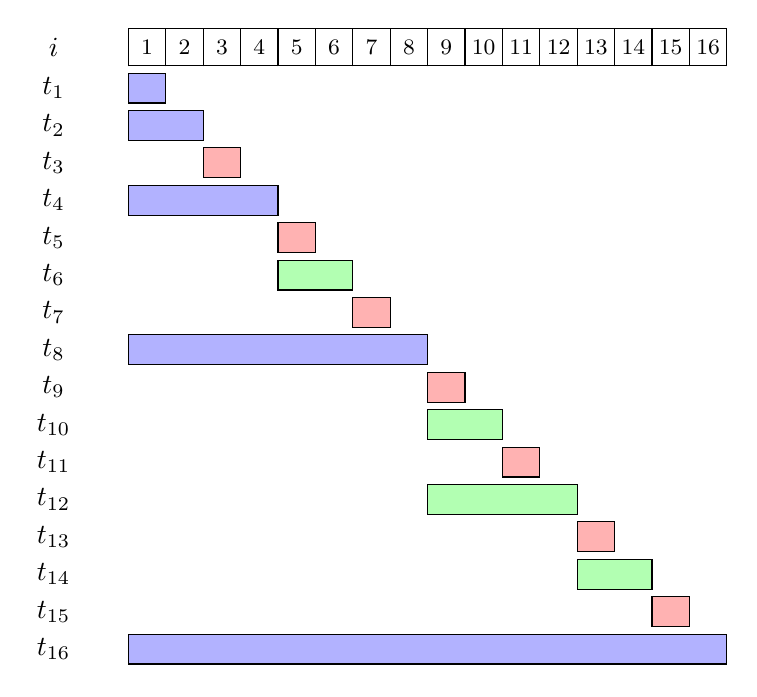
\begin{tikzpicture}[scale=0.95]
            \draw[step=0.5] (0.99999, 8.49) grid (9, 9.0);

            \node at (1.25, 8.75) { \footnotesize $1$ };
            \node at (1.75, 8.75) { \footnotesize $2$ };
            \node at (2.25, 8.75) { \footnotesize $3$ };
            \node at (2.75, 8.75) { \footnotesize $4$ };
            \node at (3.25, 8.75) { \footnotesize $5$ };
            \node at (3.75, 8.75) { \footnotesize $6$ };
            \node at (4.25, 8.75) { \footnotesize $7$ };
            \node at (4.75, 8.75) { \footnotesize $8$ };
            \node at (5.25, 8.75) { \footnotesize $9$ };
            \node at (5.75, 8.75) { \footnotesize $10$ };
            \node at (6.25, 8.75) { \footnotesize $11$ };
            \node at (6.75, 8.75) { \footnotesize $12$ };
            \node at (7.25, 8.75) { \footnotesize $13$ };
            \node at (7.75, 8.75) { \footnotesize $14$ };
            \node at (8.25, 8.75) { \footnotesize $15$ };
            \node at (8.75, 8.75) { \footnotesize $16$ };

            \node at (0, 8.75) { $i$ };
            \node at (0, 8.2) { $t_1$ };
            \node at (0, 7.7) { $t_2$ };
            \node at (0, 7.2) { $t_3$ };
            \node at (0, 6.7) { $t_4$ };
            \node at (0, 6.2) { $t_5$ };
            \node at (0, 5.7) { $t_6$ };
            \node at (0, 5.2) { $t_7$ };
            \node at (0, 4.7) { $t_8$ };
            \node at (0, 4.2) { $t_9$ };
            \node at (0, 3.7) { $t_{10}$ };
            \node at (0, 3.2) { $t_{11}$ };
            \node at (0, 2.7) { $t_{12}$ };
            \node at (0, 2.2) { $t_{13}$ };
            \node at (0, 1.7) { $t_{14}$ };
            \node at (0, 1.2) { $t_{15}$ };
            \node at (0, 0.7) { $t_{16}$ };

            \draw[fill=blue!30] (1, 8) rectangle (1.5, 8.4);
            \draw[fill=blue!30] (1, 7.5) rectangle (2, 7.9);
            \draw[fill=red!30] (2, 7.0) rectangle (2.5, 7.4);
            \draw[fill=blue!30] (1, 6.5) rectangle (3, 6.9);
            \draw[fill=red!30] (3, 6.0) rectangle (3.5, 6.4);
            \draw[fill=green!30] (3, 5.5) rectangle (4, 5.9);
            \draw[fill=red!30] (4, 5.0) rectangle (4.5, 5.4);
            \draw[fill=blue!30] (1, 4.5) rectangle (5, 4.9);
            \draw[fill=red!30] (5, 4.0) rectangle (5.5, 4.4);
            \draw[fill=green!30] (5, 3.5) rectangle (6, 3.9);
            \draw[fill=red!30] (6, 3.0) rectangle (6.5, 3.4);
            \draw[fill=green!30] (5, 2.5) rectangle (7, 2.9);
            \draw[fill=red!30] (7, 2.0) rectangle (7.5, 2.4);
            \draw[fill=green!30] (7, 1.5) rectangle (8, 1.9);
            \draw[fill=red!30] (8, 1.0) rectangle (8.5, 1.4);
            \draw[fill=blue!30] (1, 0.5) rectangle (9, 0.9);

        \end{tikzpicture}

    \end{figure}

\end{frame}

\begin{frame}[fragile]{Exemplo de representação de uma BITree em C++}
    \inputsnippet{cpp}{1}{13}{codes/ft.cpp}
\end{frame}
